\documentclass{beamer}
%[aspectratio=169]   \usepackage[czech]{babel}
\usepackage{apo-lecture}
\usepackage{pdfpages}
\usepackage{pdfcomment}
\usepackage{listings}
\usepackage{array,multirow}

\subtitle{Lekce 06. Superskalární architektura\\a\\prediktory skoků}
\author{Pavel Píša \phantom{xxxxxxxxx} Petr Štěpán \\ \small\texttt{pisa@fel.cvut.cz}\phantom{xxxx}\small\texttt{stepan@fel.cvut.cz}}
\begin{document}

\maketitle

\section{Superscalární architektura}

\begin{frame}
\frametitle{Cíl dnešní přednášky}

\begin{itemize}
 \item Podívat se na další možné zrychlení procesoru, které navazuje na pipelining
 \item Predikce skoků jako velmi důležitá vlastnost superskalárních procesorů
 \item Obě tyto techniky se využívají jak v RISC-V procesorech, tak i ve všech současných procesorech
\end{itemize}

\end{frame}

\begin{frame}

\frametitle{Procesor s pipeline (z přednášky 5)}

Jak moc je složitá Hazard Unit?
\begin{columns}
\begin{column}{0.67\textwidth}

\includegraphics[width=\textwidth]{cpu_final_design.pdf}
\end{column}
\begin{column}{0.33\textwidth}
\footnotesize
\begin{itemize}
\item Pokud je RegWriteM==1, MemToRegM==0 a WriteRegM==RsE1 nebo RsE2 pak nastav ForwardAE na 2 nebo ForwardBE na 2
\item Pokud je RegWriteW==1, MemToRegW==0 a WriteRegW==RsE1 nebo RsE2 pak nastav ForwardAE na 1 nebo ForwardBE na 1
\end{itemize}
\end{column}
\end{columns}
\bigskip
\footnotesize
\begin{itemize}
\item Pokud MemToRegM==1 a WriteRegW==Rs1E nebo Rs2E pak nastav pozastavení - STALL
\end{itemize}
\end{frame}

\begin{frame}
\frametitle{Paralelismus na úrovni instrukcí}

Paralelní zpracování na úrovni instrukcí (Instruction Level Parallelism, ILP)
\begin{itemize}
 \item Pipelining -- paralelně se zpracovávají různé fáze různých instrukcí
 \item Superskalární procesor -- paralelně se zpracovávají stejné fáze různých instrukcí
\begin{itemize}
\item můžeme mít více jednotek ALU a provádět paralelně fáze EX více různých instrukcí
\item ve fázi fetch můžeme paralelně načítat více instrukcí jdoucích po sobě, tedy instrukci z adresy PC, PC+4, PC+8 a PC+12
\item jednotlivé fáze instrukcí jsou navíc zřetězené, takže po paralelním načtení 4 instrukcí, rovnou načítáme další 4 instrukce 
\end{itemize}
\end{itemize}

\end{frame}

\begin{frame}
\frametitle{Paralelismus na úrovni instrukcí}

Zřetězený procesor -- piplened procesor
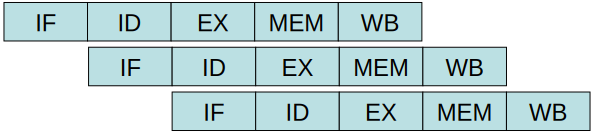
\includegraphics[width=0.85\textwidth]{pipeline.pdf}

Superskalární procesor -- super scalar procesor
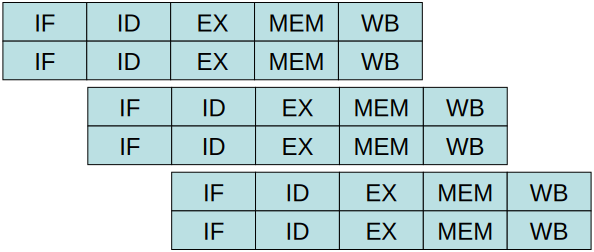
\includegraphics[width=0.85\textwidth]{superscalar.pdf}

\end{frame}

\begin{frame}
\frametitle{Superskalární procesory}

\begin{itemize}
\item Mají IPC (Instruction Per Clock) větší než 1. 
  \begin{itemize}
  \item Normální i pipelined procesor mají neustále IPC=1
  \end{itemize}
\item Počet paralelních větví se nazývá šířka zřetězení (instruction pipeline width)
\item Existují dvě základní varianty:
  \begin{itemize}
  \item \textbf{Statická} superskalární architektura -- paralelně mohou být spuštěny jen instrukce jdoucí v programu za sebou.
    \begin{itemize}
    \item Pokud na sobě instrukce závisí vede to k pozastavení procesoru (stall).
    \end{itemize}
  \item \textbf{Dynamická} superskalární architektura -- paralelně mohou být spuštěny libovolné instrukce, které jsou přiravené k vykonávání. 
    \begin{itemize}
    \item Umožňuje předbíhání instrukcí tzv. out-of-order execution.
    \item Lépe využívá HW prostředky procesoru.
    \end{itemize}
  \end{itemize}
\end{itemize}

\end{frame}

\begin{frame}
\frametitle{Superskalární procesory}

\begin{itemize}
\item Jednotlivé paralelní větve mohou být \textbf{unifikované} -- tedy všechny větve jsou stejné a mohou provádět všechny typy operací
  \begin{itemize}
  \item V praxi by to byl zbytečně složitý procesor -- nepoužívá se
  \end{itemize}
\item Jednotlivé paralelní větve jsou \textbf{specializované} -- každá větev umí jen některé instrukce:
  \begin{itemize}
  \item instrukce pracující pouze s registry -- výpočty, porovnání
  \item instrukce pracující s pamětí -- načítání/ukládání dat z/do paměti
  \item instrukce skoku -- instrukce měnící PC
  \end{itemize}
\end{itemize}
\end{frame}


\begin{frame}
\frametitle{Superskalární architektura}
\begin{columns}
\begin{column}{0.55\textwidth}
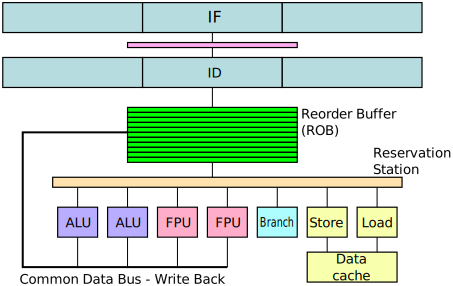
\includegraphics[width=\textwidth]{superscalar-architecture.pdf}
\end{column}
\begin{column}{0.45\textwidth}
\begin{itemize}
\item Základem architektury je ReOrder Buffer (ROB), který pomocí přejmenování registrů umí zlepšit paralelizaci instrukcí.
\item Reservation Station rozšiřuje možnosti ukládání operandů pro operace a organizuje jejich vykonávání
\item Common Data Bus zajišťuje zapsání vypočtených hodnot do skutečných registrů i pro přejmenované registry.
\end{itemize}
\end{column}
\end{columns}
\end{frame}


\begin{frame}[fragile]
\frametitle{Datové hazardy v superskalární architektuře}

Pro instrukce pracující pouze s registry:
\begin{itemize}
\item je jasné, že není možné paralelně vykonávat všechny instrukce
\item pomocí skryté sady registrů je možné paralelizaci zvýšit.
\end{itemize}

\begin{minted}[fontsize=\footnotesize]{gas}
1: slli t1, s1, 4
2: add  t0, t1, s2
3: lw   s2, 8(t0)
4: mult t1, s0, s0
5: addi t3, t1, 100
\end{minted}

Tento program lze paralelizovat s použitím skryté sady registrů pro přejmenování:

\begin{columns}[T]
\begin{column}{0.40\textwidth}
\begin{minted}[fontsize=\footnotesize]{gas}
1: slli RN0, s1, 4
2: add  RN1, RN0, s2
3: lw   s2, 8(RN1)
\end{minted}
\end{column}
\begin{column}{0.40\textwidth}
\begin{minted}[fontsize=\footnotesize]{gas}
4: mult RN2, s0, s0
5: addi RN3, RN2, 100
\end{minted}
\end{column}
\end{columns}
\end{frame}


\begin{frame}
\frametitle{Tomasulo algoritmus}

Robert Tomasulo z IBM vymyslel v roce 1967 algoritmus pro out-of-order vykonávání výpočtů na FPU.
V současné době je jeho modifikace základem architektury všech moderních procesorů.
Základní fáze jsou:
\begin{itemize}
\item Zavedení instrukce do ROB a přejmenování registru výsledku operace - získání čísla registru ze souboru záložních registrů. 
\item Zavedení instrukce do Register Station a čekání na připravená data
\item Provedení výpočtu a zapsání výsledku do přejmenovaného registru přes Common Data Bus
\item Dokončení nejstarší instrukce (kruhový buffer) z ROB a aktualizace systémového registru.
\end{itemize}
Instrukce se mohou vypočítávat out-of-order, ale ukončení instrukcí je v pořadí programu.
\end{frame}

\begin{frame}
\frametitle{Superskalární architektura}

\begin{center}
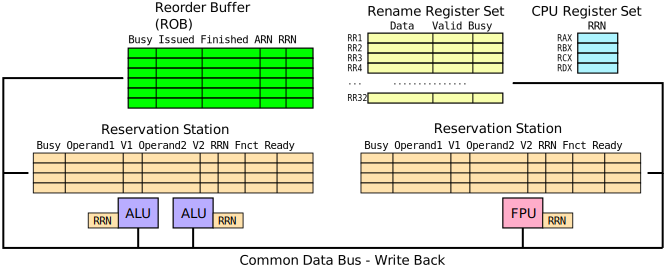
\includegraphics[width=0.7\textwidth]{superscalar-architecture2.pdf}
\end{center}

\scriptsize
Rename Register Set:
\begin{itemize}
\item Množina pomocných registrů, často až dvakrát větší než počet CPU registrů.
\item Příznak Busy značí, že registr je využíván, Příznak valid značí, že hodnota je vypočtena a je validní. Při dokončení instrukce se nastaví CPU registr na RRN.
\end{itemize}

ReOrder Buffer:
\begin{itemize}
\item Cyklická fronta obsahuje instrukce vložené v pořadí programu
\item Fronta zaručuje, že instrukce jsou dokončovány v programovém pořadí
\item Provázání mezi Reservation Station přes číslo přejmenovaného registru (RRN Rename Register Number), který bude obsahovat výsledek operace
\item Přes Common Data Bus se dozví, že registr RRN byl vypočten a instrukce dostane příznak Finished
\item Dokončení instrukce - odstraní z ROB pouze nejstarší instrukci, až získá příznak finish.
\end{itemize}


\end{frame}

\begin{frame}
\frametitle{Superskalární architektura}

\begin{center}
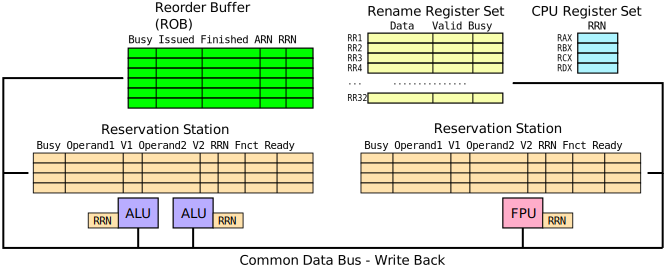
\includegraphics[width=0.7\textwidth]{superscalar-architecture2.pdf}
\end{center}

\scriptsize
Reservation Station:
\begin{itemize}
\item Obsahuje dva operandy, pokud je nastaven příznak V1/2 pak je hodnota operandu validní. Pokud není příznak V1/2 nastaven, pak operand obsahuje číslo RRN na jehož hodnotu se čeká a která přijde z CDB
\item Číslo RRN značí, do kterého registru se má zapsat výsledek.
\item Pokud jsou oba operandy validní a je volná ALU/FPU, tak se zadá provedení operace a položka se odstraní z Reservation Station (RRN výsledku se zapamatuje, aby ho ALU/FPU mohla poslat na Common Data Bus)
\end{itemize}

\end{frame}

\begin{frame}
\frametitle{Datové hazardy při čtení z paměti}

\begin{itemize}
\item Pokud instrukce lw a sw využívají jiné adresy, tak je můžeme prohazovat.
\item Pokud lw následuje po sw ze stejné adresy, lze implementovat přeposlání dat, data forwarding.
\item V praxi ale může jedna instrukce předběhnout druhou tak, že ještě není vypočteno, kam se data uloží, tedy zda dojde k hazardu.
\begin{itemize}
\item Řešení - spekulativní vykonání instrukce lw, tedy vykonání, i když není jasné, zda data budou správná
\item Při dokončování instrukce sw se zkontrolují všechny spekulativně prováděné lw 
\item Při nalezení konfliktu se zruší spekulativní provádění instrukce lw
\end{itemize}
\item Provedení se tváří, jako by bylo zachováno pořadí.
\item Velký problém v multiprocesorových systémech -- konzistence paměti při paralelních výpočtech na různých jádrech procesoru.¨
\end{itemize}

\end{frame}



\begin{frame}
\frametitle{AMD Zen2 - Mikroarchitektura}

\begin{columns}[T]
\begin{column}{0.34\textwidth}
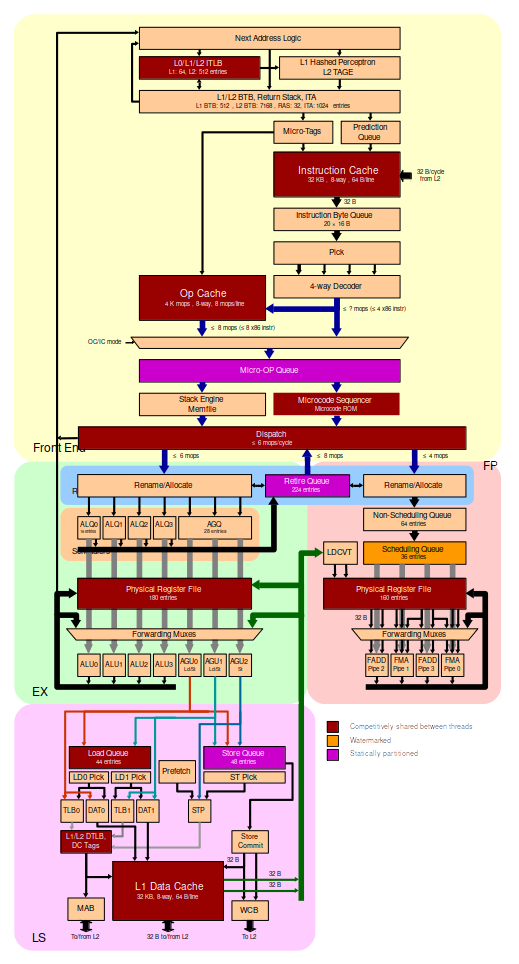
\includegraphics[width=\textwidth]{fig/amd_zen2.png}
\end{column}
\begin{column}{0.66\textwidth}
\scriptsize
\begin{itemize}
\item 7 nm process (from 12 nm), I/O die utilizes 12 nm
\item Core (8 cores on CPU chiplet),  6/8/4 µOPs in parallel
\begin{itemize}
\scriptsize
\item Frontend, µOP cache (4096 entries)
\item FPU, 256-bit Eus (256-bit FMAs) and LSU (2x256-bit L/S), 3 cycles DP vector mult latency
\item Integer, 180 registers, 3x AGU, scheduler (4x16 ALU + 1x28 AGU)
\item Reorder Buffer 224 entries
\end{itemize}
\item Memory subsystem
\begin{itemize}
\scriptsize
\item L1 i-cache and d-cache, 32 KiB each,  8-way associative
\item L2 512 KiB per core, 8-way, 
\item L2 DTLB 2048-entry
\item 48 entry store queue
\end{itemize}
\end{itemize}
Autor: QuietRub\\
Source: \url{https://en.wikichip.org/wiki/amd/microarchitectures/zen_2}
\end{column}
\end{columns}

\end{frame}


\begin{frame}
\frametitle{Řídicí hazardy v superskalární architektuře}

\begin{itemize}
\item Skoky v programu mnění, které instrukce se vykonají.
\item Při podmíněných skocích není jasné, které instrukce se budou vykonávat.
\item Výpočet podmínky pro skok může trvat dlouho, je rozpracováno mnoho instrukcí.
\begin{itemize}
\item Řešení - spekulativní nahrání dalších instrukcí
\item Po dokončení všech výpočtů nutných pro rozhodnutí skoku se ověří, zda se mělo skákat nebo ne.
\item Při chybné predikci se musí zahodit mnoho rozpracovaných, nebo i spekulativně vykonaných instrukcí.
\end{itemize}
\item I nepodmíněné skoky mají problém, vypočítat kam se skočí. Cíl skoku může záviset na výpočtu předchozích instrukcí a proto nejde jednoduše určit při načítání instrukcí.
\begin{itemize}
\item Řešení - spekulativně odhadneme, na jakou adresu se asi bude skákat, podle historie minulých skoků.
\item Po dokončení všech výpočtů se zkontroluje, zda se odhadla správná adresa.
\item Důležité zvláště pro návrat z funkce.
\end{itemize}
\end{itemize}

\end{frame}


\begin{frame}
\frametitle{Řídicí hazardy v superskalární architektuře}

\begin{itemize}
\item Skok je v programu statisticky každá 4 až 7 instrukce
\item 20\% skoků je nepodmíněných -- skočí se vždy, není potřeba rozhodovat
\item 80\% skoků je podmíněných
  \begin{itemize}
  \item asi 66\% je skoků na vyšší adresu, neboli dopředu 
    \begin{itemize}
    \item tyto skoky odpovídají větvení typu \texttt{if} 
    \item z nich statisticky asi 60\% se neskočí -- budeme značit \textbf{NT} (Not Taken)
    \end{itemize}
  \item zbytek asi 34\% je skoků na nižší adresu, neboli dozadu 
    \begin{itemize}
    \item tyto skoky odpovídají větvení typu \texttt{for}, \texttt{while} a \texttt{do ... while}
    \item z nich statisticky 99\% (téměř všechny) se skočí -- budeme značit \textbf{T} (Taken)
    \end{itemize}
  \end{itemize}
\end{itemize}

\end{frame}


\begin{frame}
\frametitle{Statické prediktory}

Statické prediktory mají pro danou skokovou instrukci vždy stejný výsledek:
\begin{itemize}
\item Prediktor, který by vždy odhadoval, že se vždy skočí 
\begin{itemize}
\item Podle statistiky z minulého slajdu by měl úspěšnost: $p_{taken} = (0.66*0.4+0.34*0.99) = 0.60$
\item Statisticky se ukazuje, že hodnota $p_{taken}$ je pro většinu programů v rozmezí 60 -- 70\%.
\end{itemize}
\item Prediktor BTFNT -- Backwards Taken / Forwards Not Taken  
\begin{itemize}
\item Podle znaménka relativního skoku - skok zpět se skočí, skok dopředu se neskočí
\item Podle statistiky z minulého slajdu by měl úspěšnost: $p_{taken} = (0.66*0.6+0.34*0.99) = 0.73$
\end{itemize}
\end{itemize}

\end{frame}


\end{document}

